\documentclass{standalone}

\usepackage{tikz}
  \usetikzlibrary{arrows}
  \usetikzlibrary{positioning}
  \usetikzlibrary{calc}
  \usetikzlibrary{backgrounds}
  \usetikzlibrary{fit}

\usepackage{fontspec}
  \setmainfont[Ligatures=TeX]{Times New Roman}

% margins
% \usepackage[margin=0cm]{geometry}

\tikzstyle{int}=[draw, fill=blue!20, minimum size=2em]
\tikzstyle{init} = [pin edge={to-,thin,black}]

\pgfdeclarelayer{background}
\pgfdeclarelayer{foreground}
\pgfsetlayers{background,main,foreground}

\begin{document}
\pagestyle{empty}



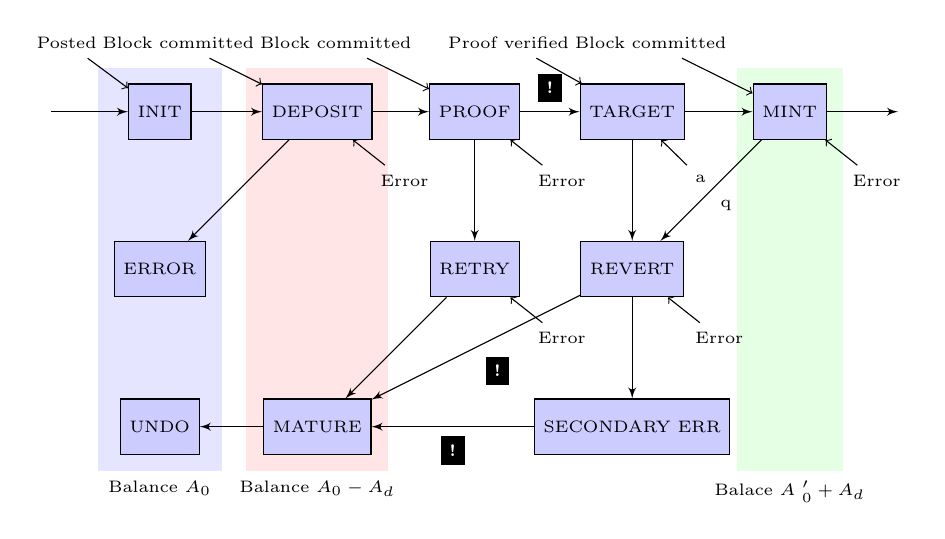
\begin{tikzpicture}[node distance=2cm,auto,>=latex']
  \tikzset{
    font={\fontsize{6pt}{8}\selectfont}
  }
    \node [int, pin={[init]above left:Posted}] (a) {INIT};
    \node (b) [left of=a,node distance=1.5cm] {};
    \node [int, pin={[init]above left:Block committed}, pin={[init]below right:Error}] (c) [right of=a] {DEPOSIT};
    \node [int, pin={[init]above left:Block committed}, pin={[init]below right:Error}] (d) [right of=c] {PROOF};
    \node [int, pin={[init]above left:Proof verified}, pin={[init]below right:a}] (e) [right of=d] {TARGET};
    \node [int, pin={[init]above left:Block committed}, pin={[init]below right:Error}] (f) [right of=e] {MINT};
    \node [] (end) [right of=f, node distance=1.5cm]{};

    \node [int] (r) [below of=a] {ERROR};
    \node [int] (r1) [below of=d, pin={[init]below right:Error}] {RETRY};
    \node [int] (m) [below of=r] {UNDO};
    \node [int] (r0) [right of=m] {MATURE};
    % \node [int] (r4) [below of=r0] {UNDO};
    \node [int] (r2) [right of=r1, pin={[init]below right:Error}] {REVERT};
    \node [int] (r3) [below of=r2] {SECONDARY ERR};
    \node [minimum size=2em] (r5) [right of=r3] {};

    \path[->] (b) edge node {} (a);
    \path[->] (a) edge node {} (c);
    \path[->] (c) edge node {} (d);
    \path[->] (d) edge node {\colorbox{black}{\textcolor{white}{\textbf{!}}}} (e);
    \path[->] (e) edge node {} (f);
    \draw[->] (f) edge node {} (end) ;

    \path[->] (c) edge node {} (r);
    \path[->] (d) edge node {} (r1);
    % \path[->] (r) edge node {} (r0);
    \path[->] (r1) edge node {} (r0);
    \path[->] (r0) edge node {} (m);
    \path[->] (e) edge node {} (r2);
    \path[->] (f) edge node {q} (r2);
    % \path[->] (r2) edge node {} (r4);
    \path[->] (r2) edge node {\colorbox{black}{\textcolor{white}{\textbf{!}}}} (r0);
    \path[->] (r2) edge node {} (r3);
    \path[->] (r3) edge node {\colorbox{black}{\textcolor{white}{\textbf{!}}}} (r0);


    % block on background of init, error and undo
    \begin{pgfonlayer}{background}
			\node [fill=blue!10,inner sep=0.2cm,fit=(a) (r) (m), label=below:Balance $A_0$ ] {};
			\node [fill=red!10,inner sep=0.2cm,fit=(c) (r0), label=below:Balance $A_0 - A_d$] {};
			\node [fill=green!10,inner sep=0.2cm,fit=(f) (r5), label=below:Balace $A~'_0 + A_d$ ] {};
	    \end{pgfonlayer}
\end{tikzpicture}

\end{document}
